\section{Formulas}
\begin{namedframe}{What's semiperimeter?}
	In order to use these next formulas, we need to know about a wonderful concept called semiperimeter.

	Semiperimeter, as the name suggests, refers to half the length of a shape's overall perimeter!

	For example, the semiperimeter of the triangle below is 12! Easy, right?
	\begin{center}
		\begin{tikzpicture}
			\coordinate (A) at (3,4);
			\coordinate (B) at (0,0);
			\coordinate (C) at (5,1);

			\draw (A) -- (B) -- (C) -- cycle;

			\tkzLabelSegment[above left](A,B){$10$};
			\tkzLabelSegment[below right](B,C){$8$};
			\tkzLabelSegment[above right](A,C){$6$};
		\end{tikzpicture}
	\end{center}
\end{namedframe}
\begin{namedframe}{Heron's formula: a neat way to calculate area!}
	A formula that can be used to calculate the area of triangles using semiperimeter!
	\sep
	The formula is:
	\[A = \sqrt{s(s - a)(s-b)(s-c)}\]
	Where:
	\begin{description}
		\item[$A$] is the area
		\item[$s$] is the semiperimeter
		\item[$a$, $b$, and $c$] are the sides of the triangle
	\end{description}
\end{namedframe}
\begin{namedframe}{More triangles and semiperimeters!}
	The area of a triangle is also the product of a circle's inradius and its semiperimeter, or $A=rs$.

	A triangle's inradius refers to the radius of its incircle, or the circle that can be inscribed within the triangle.
	\begin{center}
		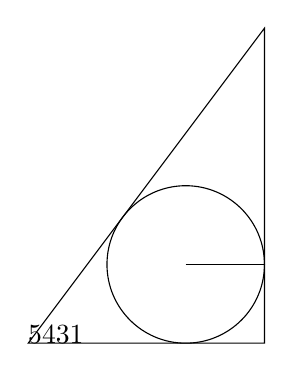
\begin{tikzpicture}
			\coordinate (A) at (0,0);
			\coordinate (B) at (3,4);
			\coordinate (C) at (3,0);
			\coordinate (D) at (2,1);
			\coordinate (E) at (3,1);

			\draw (A) -- (B) -- (C) -- cycle;

			\draw (D) circle (1);
			\draw (D) -- (E);

			\tkzLabelSegment[above left](A,B){$5$};
			\tkzLabelSegment[right](B,C){$4$};
			\tkzLabelSegment[below](A,C){$3$};

			\tkzLabelSegment[above](D,E){$1$};
		\end{tikzpicture}
	\end{center}
\end{namedframe}
\begin{namedframe}{Another formula}
	Here's a formula that can be used to calculate the circumradius!
	\[R = \frac{abc}{4\sqrt{s(s-a)(s-b)(s-c)}} = \frac{abc}{4A}\]
	A circumradius refers to, you can probably guess, the radius of the circle that the triangle can be inscribed in!
	\begin{center}
		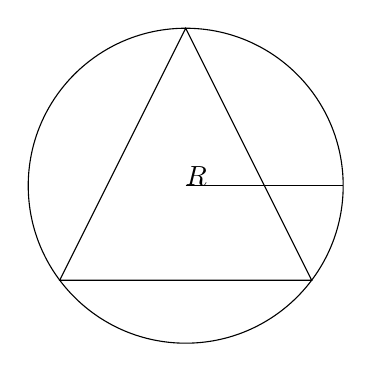
\begin{tikzpicture}[scale=0.4]
			\coordinate (A) at (0,5);
			\coordinate (B) at (-4,-3);
			\coordinate (C) at (4,-3);
			\coordinate (D) at (0,0);
			\coordinate (E) at (5,0);

			\draw (D) circle (5);

			\draw (A) -- (B) -- (C) -- cycle;

			\draw (D) -- (E);
			\tkzLabelSegment[above right](D,E){$R$};
		\end{tikzpicture}
	\end{center}
\end{namedframe}
\begin{namedframe}{Brahmagupta's Formula: The key to cyclic quads}
	Similarly to Heron's formula, Brahmagupta's formula is another way to calculate area, however it involves the semiperimeter of a cyclic quadrilateral!

	Remember: a cyclic quadrilateral is a quadrilateral where all of the vertices lie on one circle.
	\sep
	The formula is:
	\[K = \sqrt{(s-a)(s-b)(s-c)(s-d)}\]
	Where:
	\begin{description}
		\item[$K$] is the area
		\item[$s$] is the semiperimeter
		\item[$a$, $b$, $c$, and $d$] are the sides of the quadrilateral
	\end{description}
\end{namedframe}
